\documentclass{article}
\usepackage{amsmath}
\usepackage{tikz}
% Title
\author{Daniel Bustos}
\title{Ejercicio 4: Arte Conexo}

\begin{document}
\section{Arte Conexo}
\textbf{Daniel Bustos}
\subsection{a)}
Sea $G = (V,E)$ un grafo, con $|V| = n$. \\
Sea $P(n)$ := Si un grafo tiene más de $\frac{(n-1) \cdot (n-2)}{2}$ aristas $\rightarrow$ es conexo. \\

\textbf{Caso Base}: $P(1) =$ Tenemos $1$ vértice, con $0$ aristas: Se falsea el antecedente, luego $P(1)$ es verdadero. \\

\textbf{Paso inductivo}: \textbf{H.I}: Supongamos que existe un $n_0$ tal que para todo Grafo con $n_0$ vértices que tenga más de $\frac{(n_0 - 1) \cdot (n_0 - 2)}{2}$ aristas $->$ es conexo. \\

\textbf{Q.V.Q}: $P(n_0) -> P(n_0  + 1)$ \\

Tenemos un grafo $G$ con $n_0 + 1$ vértices, queremos probar que si tiene más de $\frac{n_0 \cdot (n_0-1)}{2}$ aristas $->$ es conexo.
\begin{itemize}

	\item Si tiene menor o igual a la cantidad de aristas pedida, entonces se falsea el antecedente, haciendo verdadera a la propiedad:
	
	\item \textbf{Observemos} que no puede haber ningun vertice de grado 0 en G. Probemoslo rapidamente por el absurdo: Supongamos $\exists v \in V d(v) = 0$ \\ 
	Podemos considerar el grafo $G-\{v\}$ que tendra $n_0$ vertices y la misma cantidad de aristas que G, ya que d(v) = 0. Dado que tiene $n_0$ vertices, $G-\{v\}$ podra tener como maximo :$ \binom{n_0}{2} = \frac{(n_0) \cdot (n_0-1)}{2}$ aristas.\\ \\
	Pero dijimos que $G-\{v\}$ tiene  estrictamente mas de esa cantidad!(Recordemos G  y $G-\{v\}$ tienen la misma cantidad de aristas). Luego no puede existir en G un vertice de grado 0.
		  
    \item Si hay un nodo $v$ de  grado $1$, podemos considerar el grafo $G-v$. Este tiene $n_0$ nodos y $\frac{n_0 \cdot (n_0 -1)}{2}  - 1$ aristas. Observemos que: 
    $$\frac{n_0 \cdot (n_0 -1)}{2}  - 1 > \frac{(n_0-1) \cdot (n_0-2)}{2}$$ 
    Luego tenemos un grafo que cumple la H.I por lo tanto es $G-\{v\}$ es conexo . Como $G-\{v\}$ es subgrafo de G y conexo,  dado que el vertice v tiene mas de grado 0, G debe ser conexo tambien.Por lo tanto es verdadero $P(n_0 + 1)$ en este caso.
    
    \item ¿Hasta qué grado de nodo podemos remover, tal que siga valiendo la desigualdad de la H.I.? Plantemos la desigualdad. Sea $a$ el grado mayor del nodo que podemos sacar.
    \begin{align*}
        &\frac{n_0 \cdot (n_0 -1)}{2}  - a > \frac{(n_0-1) \cdot (n_0-2)}{2} \\
        &\leftrightarrow \left(\frac{n_0^2}{2} -\frac{n_0}{2} - a\right) > \left(\frac{n_0^2}{2} - \frac{2n_0}{2} - \frac{n_0}{2} + \frac{2}{2}\right) \\
        &\leftrightarrow -\frac{n_0}{2}  -a > - \frac{3}{2}n_0 + 1 \\
        &\leftrightarrow n_0 - a > 1 \\
        &\leftrightarrow n_0 - 1 > a
    \end{align*}
   Luego podemos sacar nodos de hasta grado $n_0 - 2$, y generarnos un Grafo de $n_0$ vertices que  cumpla la desigualdad, haciendo valer la H.I y por ende demostrando que G es conexo a partir del mismo razonamiento que hicimos antes.
   \item ¿Pero qué pasa si todos los nodos tienen grado $n_0-1$? 
   ¡Fácil! Si todos los nodos tienen grado $n_0 -1$, entonces el grafo es conexo por definición, ya que es completo (todos están conectados con todos).
\end{itemize}    

Luego vimos que $P(n_0 +1)$ vale para todos los casos. 
Por lo tanto $P(n)$ vale $\forall n \geq 0$.

\newpage



\subsection{b)}

Sea $G = (V,E)$ un grafo $(|V| = n)$ tal que: $|E| \geq 2 + \frac{(n-1)(n-2)}{2}$ aristas. Queremos ver que si tiene esa cantidad de aristas entonces es biconexo.\\ \\
Sabemos por el inciso (a) que $\forall G'$ si $|E'| > \frac{(n-1)(n-2)}{2}  \rightarrow G'$ es conexo.\\

\textbf{Q.V.Q}: $G$ es biconexo.\\

Supongamos que $G$ no es biconexo $\rightarrow \exists v \in V$ tal que $v$ es articulación  $(G-v$ tiene mas partes conexas que $G)$.

Por la propiedad de (a) sabemos que necesariamente $G$ es conexo ya que:

\[ |E| \geq 2 + \frac{(n-1)(n-2)}{2} > \frac{(n-1)(n-2)}{2} \]

Luego se debe cumplir que $G - v$ tiene al menos dos partes conexas o lo que es lo mismo, $G-v$ no puede ser conexo.

¿Qué grado debe tener $v$ para que se cumpla esto? Sabemos que el grafo $G-v$ tiene $n - 1$ vertices , luego debe cumplir que:

\[ |E(G-v)| \leq \frac{(n-2)(n-3)}{2} \]
Ya que de otra forma seria conexo por la propiedad (a).

Veamos ahora si esto es en efecto posible:

\[ |E(G-v)| = |E| - d(v) \geq 2 + \frac{(n-1)(n-2)}{2} - d(v)  \leq (Q.V.Q) \frac{(n-2)(n-3)}{2} \]
\[ \leftrightarrow 2 + \frac{(n-1)(n-2)}{2} - d(v)  \leq \frac{(n-2)(n-3)}{2}  \]
\[ \leftrightarrow 2 + \frac{n^2}{2} - n - \frac{n}{2} + 1 -d(v) \leq \frac{n^2}{2} - \frac{3n}{2} - n + 3 \]
\[ \leftrightarrow 3 - \frac{3n}{2}  - d(v) \leq -\frac{5n}{2} + 3 \]
\[ \leftrightarrow 3 + n - d(v) \leq 3 \]
\[ \leftrightarrow n \leq d(v) \text{ ABS!!!} \]

Ya que el grado de un nodo tiene como cota superior $n-1$, llegamos a un absurdo. Luego $v$ no puede existir, es decir $G$ no tiene articulación.

Por lo tanto, $G$ es biconexo, probando lo que queríamos demostrar.

\newpage
\subsection{c)}





Probemos que es imposible por contraejemplo:

\textbf{1er caso)} sea $c(n) < 1 + \frac{(n-1)(n-2)}{2}$ tal que $\forall G$ grafos con $n \geq n_0$ que tenga al menos $c(n)$ aristas sea conexo.
Sabemos que c(n) debe ser : $c(n) \leq \frac{(n-1)(n-2)}{2}$ \\

Si $n = 3$: $c(3) \leq 1$. Pero podemos dibujar el grafo:
\begin{center}
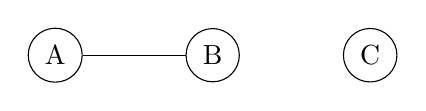
\begin{tikzpicture}
    \node[circle,draw] (A) at (0,0) {A};
    \node[circle,draw] (B) at (2,0) {B};
    \node[circle,draw] (C) at (4,0) {C};
    \draw (A) -- (B);
\end{tikzpicture}
\end{center}
que tiene una arista, sin embargo claramente no es conexo.Luego c(n) no puede existir

\textbf{2do caso)} sea $c(n) < 2 + \frac{(n-1)(n-2)}{2}$ tal que $\forall G$ grafos con $n \geq n_0$ que tenga al menos $c(n)$ aristas sea biconexo.\\
Sabemos que c(n) debe ser : $c(n) \leq 1 + \frac{(n-1)(n-2)}{2}$ \\

Si $n = 3$: $c(3) \leq 4$ pero podemos dibujar el grafo:
\begin{center}
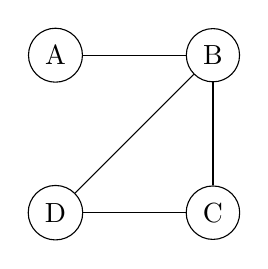
\begin{tikzpicture}
    \node[circle,draw] (A) at (0,0) {A};
    \node[circle,draw] (B) at (2,0) {B};
    \node[circle,draw] (C) at (2,-2) {C};
    \node[circle,draw] (D) at (0,-2) {D};
    \draw (A) -- (B);
    \draw (B) -- (C);
    \draw (B) -- (D);
    \draw (C) -- (D);
\end{tikzpicture}
\end{center}
que claramente es conexo, pero B es un vértice de articulación, luego no es biconexo y c(n) no puede existir



\end{document}
